\chapter{A Hybrid Transformer-LSTM Model for Fault Diagnosis}
\label{cha:hybrid_model}

\section{Overall Model Architecture}
\label{sec:hybrid_model:architecture}

\subsection{Model Overview and Data Flow}

The core of this research is the \texttt{TransformerLSTMModel}, a deep learning hybrid architecture specifically designed to extract multi-level temporal features from sequential data for classification tasks. This approach combines the global attention capabilities of Transformer networks \citep{vaswani2017attention} with the sequential modeling strengths of LSTM architectures \citep{hochreiter1997long}, creating a powerful framework for fault diagnosis applications \citep{zhang2019deep, zhao2019deep}. Figure~\ref{fig:hybrid_architecture} illustrates the complete architecture of our proposed model.

\begin{figure}[htbp]
\centering
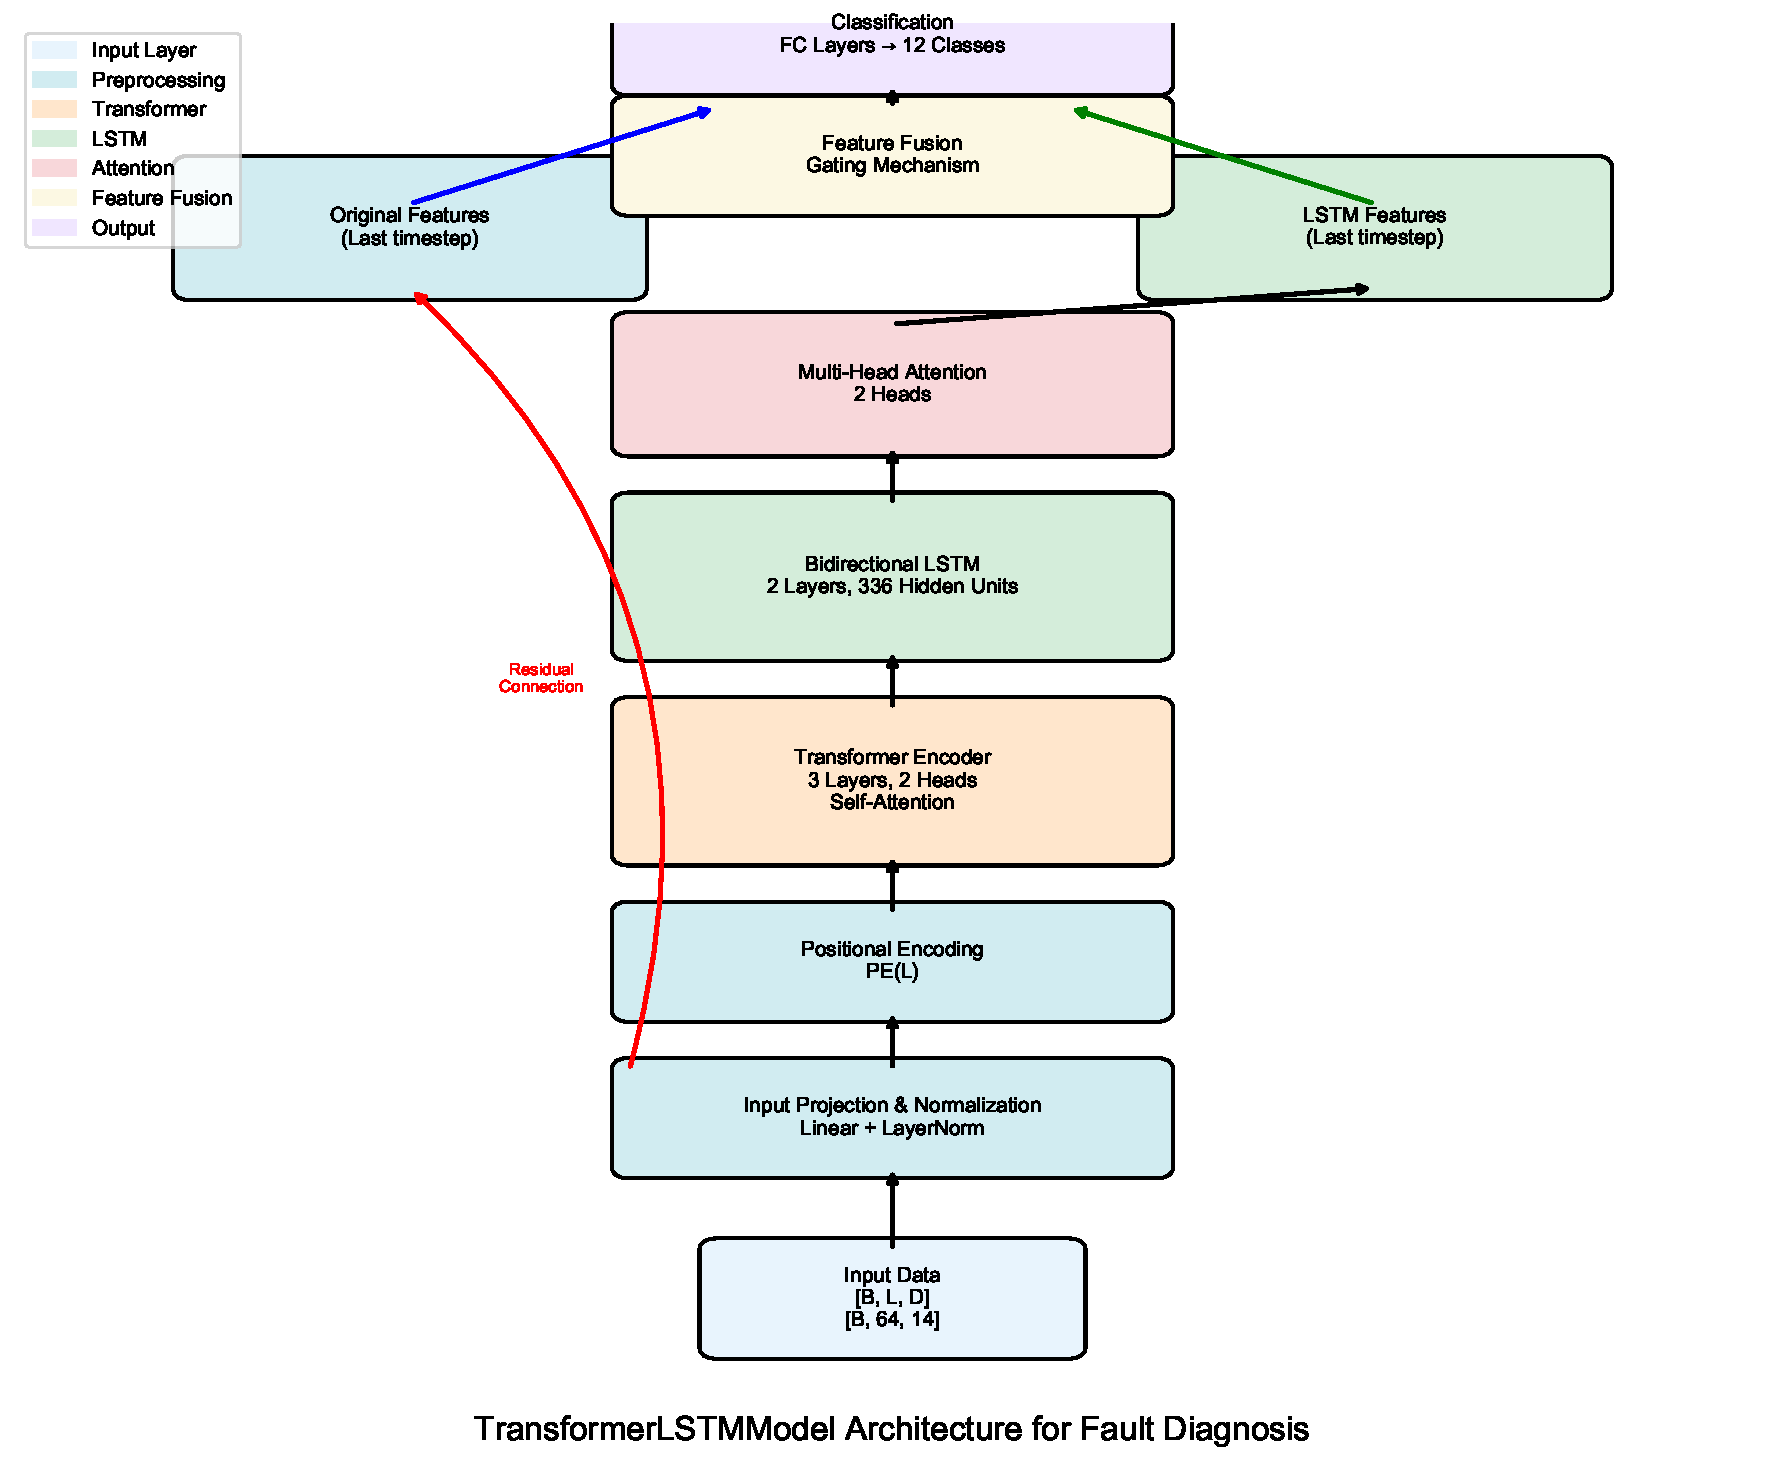
\includegraphics[width=0.9\textwidth]{logos/hybrid_architecture.pdf}
\caption{TransformerLSTMModel Architecture Overview: The diagram shows the complete data flow from input time-series data through various processing stages including input projection, positional encoding, Transformer encoder, bidirectional LSTM, multi-head attention, and feature fusion, ultimately leading to fault classification.}
\label{fig:hybrid_architecture}
\end{figure}

The model processes input data through a carefully designed pipeline that leverages the complementary strengths of Transformer and LSTM architectures. The data processing pipeline operates as follows:

\begin{enumerate}
    \item \textbf{Input Data}: Raw time-series data, typically with a shape of \texttt{[batch\_size, sequence\_length, feature\_dimension]}.
    \item \textbf{Input Projection \& Normalization}: The input data is first projected through a linear layer and then subjected to Layer Normalization \citep{ba2016layer}. This step helps stabilize the distribution of input features, preparing them for the subsequent Transformer layers.
    \item \textbf{Positional Encoding}: Since the Transformer model is inherently permutation-invariant and lacks the ability to process sequence order \citep{vaswani2017attention}, positional encodings are added to the input data. This allows the model to understand the relative or absolute position of each time step in the sequence.
    \item \textbf{Transformer Encoder}: The positionally-encoded input is fed into the Transformer Encoder. Through its self-attention mechanism \citep{bahdanau2015neural, vaswani2017attention}, the Transformer layer captures long-range dependencies and global contextual information within the sequence. It can process the entire sequence in parallel, efficiently discovering complex relationships between different time steps.
    \item \textbf{LSTM Layer}: The output from the Transformer Encoder is then passed to a Bidirectional Long Short-Term Memory (LSTM) network \citep{hochreiter1997long}. The LSTM layer excels at processing local temporal dependencies and patterns in sequential data, addressing the vanishing gradient problem in traditional RNNs \citep{pascanu2013difficulty}. The bidirectional nature allows the model to consider both past and future contexts, further enhancing its understanding of the sequence dynamics.
    \item \textbf{Multihead Attention}: The output of the LSTM layer is processed by another Multihead Attention mechanism \citep{vaswani2017attention}. This attention layer operates on the LSTM's output sequence, aiming to further refine and weigh the temporal features extracted by the LSTM, thereby focusing on the information most critical for the classification task.
    \item \textbf{Feature Fusion}: This is a critical fusion stage. The model concatenates the feature from the final time step of the attention-processed LSTM output with the feature from the final time step of the projected and normalized original input. Subsequently, a gating mechanism (\texttt{feature\_gate}) adaptively adjusts and fuses these features from different processing stages. This fusion strategy allows the model to combine the global perspective of the Transformer with the local temporal insights of the LSTM, while also leveraging direct information from the raw features.
    \item \textbf{Fully Connected Layers}: The fused features are fed into a series of fully connected layers. These layers are responsible for mapping the extracted and fused high-level features to the final class output space.
    \item \textbf{Output}: The final output of the model, typically a probability distribution over the predicted classes.
\end{enumerate}

\subsection{Core Design Philosophy: Divide and Conquer, Leveraging Strengths}

The core design philosophy of this model architecture is "divide and conquer, leveraging individual strengths," which involves fully utilizing the respective advantages of the Transformer and LSTM and combining them through an effective fusion mechanism to achieve a more comprehensive and robust analysis of time-series data.

\begin{itemize}
    \item \textbf{Transformer: Global Dependencies and Parallel Processing}
    \begin{itemize}
        \item \textbf{Strengths:} The Transformer, through its self-attention mechanism, can efficiently capture long-range dependencies between any two positions in a sequence, regardless of their distance \citep{vaswani2017attention, shaw2018self}. This is crucial for understanding global patterns and context. Furthermore, its parallel computation capability provides a significant efficiency advantage when processing long sequences, addressing limitations of sequential models like traditional RNNs \citep{pascanu2013difficulty}.
        \item \textbf{Role:} In this architecture, the Transformer is primarily responsible for performing global feature extraction and contextual modeling on the input sequence at an early stage, providing a representation enriched with global information for the subsequent LSTM layer.
    \end{itemize}
    \item \textbf{LSTM: Local Temporal Patterns and Memory}
    \begin{itemize}
        \item \textbf{Strengths:} As a recurrent neural network, the LSTM possesses excellent memory capabilities for processing sequential data, enabling it to effectively learn and remember local temporal patterns and short-term dependencies \citep{hochreiter1997long}. The bidirectional nature further enhances this ability by allowing it to consider both past and future information, making it particularly suitable for time-series analysis in fault diagnosis applications \citep{filonov2016multivariateindustrialtimeseries, zhao2019deep}.
        \item \textbf{Role:} The role of the LSTM in this architecture is to further refine and capture more fine-grained local temporal features and dynamic changes, building upon the global features extracted by the Transformer. It deeply models the sequential nature of the information.
    \end{itemize}
    \item \textbf{Fusion Mechanism: Synergy and Information Integration}
    \begin{itemize}
        \item \textbf{Strengths:} A simple serial connection might not fully realize the synergy between the two models. This model implements a more intelligent information integration by introducing another attention mechanism after the LSTM output and incorporating a gated fusion with the original input features. This fusion not only combines the global perspective of the Transformer and the local insights of the LSTM but also adaptively adjusts the importance of features from different sources via the gating mechanism, ensuring effective information transfer and complementarity.
        \item \textbf{Role:} The fusion mechanism ensures that the model can learn from different levels and types of features, thereby constructing a more powerful and discriminative feature representation that ultimately enhances the overall performance of the model.
    \end{itemize}
\end{itemize}

Through this "divide and conquer, leveraging strengths" design, the \texttt{TransformerLSTMModel} can effectively process complex time-series data, capturing both long-range dependencies and global context while finely modeling local temporal patterns, ultimately achieving high-precision classification.

\subsection{Mathematical Formulation}
\label{subsec:mathematical_formulation}

To provide a formal mathematical description of the model architecture, we define the sequential transformations applied to the input data. Given an input time-series sequence $X \in \mathbb{R}^{B \times L \times D}$, where $B$ represents the batch size, $L$ denotes the sequence length (typically 64), and $D$ is the feature dimension (14 for our fault diagnosis dataset), the model processes the data through the following stages:

\begin{align}
X_{\text{proj}} &= \text{LayerNorm}(\text{Linear}(X)) \label{eq:input_projection} \\
X_{\text{pos}} &= X_{\text{proj}} + \text{PE}(L) \label{eq:positional_encoding} \\
H_{\text{trans}} &= \text{TransformerEncoder}(X_{\text{pos}}) \label{eq:transformer} \\
H_{\text{lstm}} &= \text{BiLSTM}(H_{\text{trans}}) \label{eq:lstm} \\
H_{\text{attn}} &= \text{MultiHeadAttention}(H_{\text{lstm}}, H_{\text{lstm}}, H_{\text{lstm}}) \label{eq:attention} \\
H_{\text{fused}} &= \text{FeatureGate}([H_{\text{attn}}[-1], X_{\text{proj}}[-1]]) \label{eq:fusion} \\
\hat{y} &= \text{FC}(H_{\text{fused}}) \label{eq:output}
\end{align}

where $\text{PE}(L)$ represents the sinusoidal positional encoding, $H_{\text{attn}}[-1]$ and $X_{\text{proj}}[-1]$ denote the final time-step features from the attention output and projected input respectively, and $\text{FC}$ represents the fully connected classification layers.

The feature gating mechanism is defined as:
\begin{align}
\text{FeatureGate}(h_{\text{attn}}, h_{\text{orig}}) &= h_{\text{attn}} \odot \sigma(\text{Linear}([h_{\text{attn}}, h_{\text{orig}}])) \label{eq:gate}
\end{align}

where $\odot$ denotes element-wise multiplication, $\sigma$ is the sigmoid activation function, and $[\cdot, \cdot]$ represents concatenation.

\subsection{Model Configuration and Parameters}
\label{subsec:model_configuration}

Table~\ref{tab:model_config} presents the specific configuration parameters used in our \texttt{TransformerLSTMModel} implementation, optimized for fault diagnosis tasks.

\begin{table}[htbp]
\centering
\caption{TransformerLSTMModel Configuration Parameters}
\label{tab:model_config}
\begin{tabular}{|l|c|l|}
\hline
\textbf{Component} & \textbf{Parameter} & \textbf{Value} \\
\hline
\multirow{2}{*}{Input Processing} & Input Dimension & 14 \\
 & Sequence Length & 64 \\
\hline
\multirow{4}{*}{Transformer Encoder} & Hidden Dimension & 336 \\
 & Number of Layers & 3 \\
 & Number of Attention Heads & 2 \\
 & Dropout Rate & 0.22 \\
\hline
\multirow{3}{*}{LSTM Component} & Hidden Units & 336 \\
 & Number of Layers & 2 \\
 & Bidirectional & True \\
\hline
\multirow{2}{*}{Attention Mechanism} & Embed Dimension & 672 (336$\times$2) \\
 & Number of Heads & 2 \\
\hline
\multirow{3}{*}{Classification Layers} & FC1 Dimension & 336 \\
 & FC2 Dimension & 168 \\
 & Output Classes & 12 \\
\hline
\multirow{2}{*}{Training} & Learning Rate & 0.0006 \\
 & Weight Decay & 6$\times$10$^{-5}$ \\
\hline
\end{tabular}
\end{table}

The model contains approximately 2.1 million trainable parameters, making it computationally efficient while maintaining high representational capacity for complex fault pattern recognition.

\subsection{Computational Complexity Analysis}
\label{subsec:complexity_analysis}

The computational complexity of the \texttt{TransformerLSTMModel} can be analyzed by examining each component:

\begin{itemize}
    \item \textbf{Transformer Encoder}: The self-attention mechanism has complexity $O(L^2 \cdot D)$ for sequence length $L$ and hidden dimension $D$. With 3 layers, the total complexity is $O(3 \cdot L^2 \cdot D)$.
    
    \item \textbf{LSTM Processing}: The bidirectional LSTM with 2 layers has complexity $O(2 \cdot L \cdot D^2)$ for sequential processing.
    
    \item \textbf{Multi-head Attention}: The final attention layer adds $O(L^2 \cdot D_{lstm})$ complexity, where $D_{lstm} = 2D$ for bidirectional LSTM.
    
    \item \textbf{Overall Complexity}: The total computational complexity is $O(L^2 \cdot D + L \cdot D^2)$, which scales quadratically with sequence length but remains manageable for our typical sequence length of 64.
\end{itemize}

For our specific configuration with $L = 64$ and $D = 336$, this results in efficient processing suitable for real-time fault diagnosis applications.

\section{Data Preprocessing Module}
\label{sec:hybrid_model:preprocessing}

The data preprocessing module is a critical component that prepares raw machine fault data for effective learning by the hybrid model. This module encompasses several key operations designed to enhance data quality, increase dataset diversity, and ensure optimal model performance \citep{zhang2019deep, liu2018artificial}.

\subsection{Data Loading and Class Merging}
\label{subsec:data_loading}

Our fault diagnosis system processes 12 distinct fault categories as defined in the label set:
\begin{align}
\mathcal{L} = \{&\text{good, JERK\_A, BACKLASH\_X, JERK\_ALL,} \nonumber \\
&\text{ALL, JERK\_X, BACKLASH\_Y, BS\_XY,} \nonumber \\
&\text{BS\_X, JERK\_Y, JERK\_B, BS\_Y}\}
\end{align}

The preprocessing module consolidates multiple ``good'' condition files (good\_1, good\_2, good\_3) into a single normal operating class, ensuring balanced representation of healthy machine states across different operational scenarios.

\subsection{Sliding Window Sequence Generation}
\label{subsec:sliding_window}

To capture temporal patterns essential for fault diagnosis, the preprocessing module implements an adaptive sliding window approach:

\begin{itemize}
    \item \textbf{Window Size}: Fixed at 64 time steps, optimized for capturing both short-term transients and medium-term fault development patterns
    \item \textbf{Sampling Strategy}: For longer sequences (> 192 samples), up to 800 windows are randomly sampled per file to maximize data utilization while maintaining computational efficiency
    \item \textbf{Overlap Management}: Random starting positions prevent systematic bias and ensure diverse temporal perspectives of fault patterns
\end{itemize}

The sliding window extraction process can be formalized as:
\begin{align}
W_i &= X[s_i : s_i + L] \quad \text{for } i = 1, 2, \ldots, N_w \\
s_i &\sim \text{Uniform}(0, T - L)
\end{align}
where $W_i$ represents the $i$-th window, $s_i$ is the starting position, $L = 64$ is the window length, $T$ is the total sequence length, and $N_w$ is the number of windows extracted.

\subsection{Data Normalization and Scaling}
\label{subsec:normalization}

To ensure numerical stability and convergence, the preprocessing module employs robust scaling techniques:

\begin{itemize}
    \item \textbf{Robust Scaler}: Applied to handle outliers and maintain signal characteristics across different sensors and operational conditions
    \item \textbf{Channel-wise Normalization}: Each of the 14 sensor channels is independently scaled to preserve relative signal relationships
    \item \textbf{Preservation of Temporal Dependencies}: Scaling parameters are computed globally but applied consistently to maintain temporal coherence
\end{itemize}

The robust scaling transformation is defined as:
\begin{equation}
X_{\text{scaled}} = \frac{X - \text{median}(X)}{\text{IQR}(X)}
\end{equation}
where IQR represents the interquartile range, providing robustness against outliers commonly present in industrial sensor data.

\subsection{Data Augmentation Strategies}
\label{subsec:data_augmentation}

To enhance model generalization and address class imbalance, the preprocessing module incorporates several augmentation techniques:

\begin{enumerate}
    \item \textbf{Amplitude Scaling}: Random scaling factors $\alpha \sim \mathcal{U}(0.85, 1.15)$ applied channel-wise with 70\% probability
    \item \textbf{Gaussian Noise Injection}: Low-level noise $\epsilon \sim \mathcal{N}(0, 0.01\sigma^2)$ added to simulate sensor uncertainty  
    \item \textbf{Time Shifting}: Minimal temporal shifts to account for synchronization variations
    \item \textbf{Channel Dropout}: Random masking of sensor channels to improve robustness against sensor failures
\end{enumerate}

These augmentation strategies are applied probabilistically during training to increase dataset diversity while preserving the fundamental characteristics of fault signatures.

\section{Transformer Feature Extraction Component}
\label{sec:hybrid_model:transformer_component}

The Transformer component serves as the global feature extraction backbone of our hybrid architecture, leveraging self-attention mechanisms to capture long-range dependencies and global patterns within the fault signature sequences \citep{vaswani2017attention, zhou2021informer}.

\subsection{Input Processing and Positional Encoding}
\label{subsec:input_processing}

The Transformer component begins with input processing that prepares the sequential data for attention-based feature extraction:

\begin{enumerate}
    \item \textbf{Input Projection}: A linear transformation projects the 14-dimensional sensor readings into the model's hidden dimension:
    \begin{equation}
    X_{\text{proj}} = X \cdot W_{\text{proj}} + b_{\text{proj}}
    \end{equation}
    where $W_{\text{proj}} \in \mathbb{R}^{14 \times 336}$ and $X_{\text{proj}} \in \mathbb{R}^{B \times 64 \times 336}$.
    
    \item \textbf{Layer Normalization}: Applied to stabilize training and improve convergence:
    \begin{equation}
    X_{\text{norm}} = \text{LayerNorm}(X_{\text{proj}})
    \end{equation}
    
    \item \textbf{Sinusoidal Positional Encoding}: Since Transformers lack inherent sequential processing, positional information is added:
    \begin{align}
    PE_{(pos, 2i)} &= \sin\left(\frac{pos}{10000^{2i/d_{model}}}\right) \\
    PE_{(pos, 2i+1)} &= \cos\left(\frac{pos}{10000^{2i/d_{model}}}\right)
    \end{align}
    where $pos$ is the position, $i$ is the dimension index, and $d_{model} = 336$.
\end{enumerate}

\subsection{Multi-Head Self-Attention Mechanism}
\label{subsec:self_attention}

The core of the Transformer component employs multi-head self-attention to capture complex relationships between different time steps in the fault signature:

\begin{align}
\text{Attention}(Q, K, V) &= \text{softmax}\left(\frac{QK^T}{\sqrt{d_k}}\right)V \\
\text{MultiHead}(X) &= \text{Concat}(\text{head}_1, \ldots, \text{head}_h)W^O
\end{align}

where each attention head is computed as:
\begin{equation}
\text{head}_i = \text{Attention}(XW_i^Q, XW_i^K, XW_i^V)
\end{equation}

With 2 attention heads and $d_k = d_v = 168$, the mechanism enables the model to attend to different types of temporal relationships simultaneously.

\subsection{Feed-Forward Networks and Residual Connections}
\label{subsec:ffn_residual}

Each Transformer layer incorporates position-wise feed-forward networks with residual connections:

\begin{align}
\text{FFN}(x) &= \text{ReLU}(xW_1 + b_1)W_2 + b_2 \\
\text{TransformerLayer}(x) &= \text{LayerNorm}(x + \text{FFN}(\text{LayerNorm}(x + \text{MultiHead}(x))))
\end{align}

The residual connections facilitate gradient flow during training, while layer normalization ensures stable optimization dynamics.

\subsection{Global Context Extraction}
\label{subsec:global_context}

Through 3 stacked Transformer layers, the component progressively builds representations that capture:

\begin{itemize}
    \item \textbf{Short-term Correlations}: Direct dependencies between adjacent time steps
    \item \textbf{Medium-term Patterns}: Periodic behaviors and cyclic fault signatures  
    \item \textbf{Long-range Dependencies}: Global trends and slowly evolving fault characteristics
    \item \textbf{Cross-channel Interactions}: Relationships between different sensor modalities
\end{itemize}

The parallel processing capability of the Transformer enables efficient computation while maintaining the ability to model complex temporal interactions essential for accurate fault diagnosis.

\section{LSTM Sequence Modeling Component}
\label{sec:hybrid_model:lstm_component}

The LSTM component operates on the globally-enhanced representations from the Transformer, focusing on sequential pattern extraction and local temporal dependency modeling. This component is specifically designed to capture the recurrent nature of fault evolution and machine degradation processes \citep{hochreiter1997long, filonov2016multivariateindustrialtimeseries}.

\subsection{Bidirectional LSTM Architecture}
\label{subsec:bilstm_architecture}

The LSTM component employs a bidirectional architecture with 2 layers, each containing 336 hidden units. The bidirectional design enables the model to process information from both past and future contexts:

\begin{align}
\overrightarrow{h}_t &= \text{LSTM}_{\text{forward}}(x_t, \overrightarrow{h}_{t-1}) \\
\overleftarrow{h}_t &= \text{LSTM}_{\text{backward}}(x_t, \overleftarrow{h}_{t+1}) \\
h_t &= [\overrightarrow{h}_t; \overleftarrow{h}_t]
\end{align}

where $h_t \in \mathbb{R}^{672}$ represents the concatenated bidirectional hidden state at time step $t$.

\subsection{LSTM Cell Dynamics}
\label{subsec:lstm_dynamics}

Each LSTM cell implements the standard gating mechanism to control information flow \citep{hochreiter1997long}:

\begin{align}
f_t &= \sigma(W_f \cdot [h_{t-1}, x_t] + b_f) \quad \text{(forget gate)} \\
i_t &= \sigma(W_i \cdot [h_{t-1}, x_t] + b_i) \quad \text{(input gate)} \\
\tilde{C}_t &= \tanh(W_C \cdot [h_{t-1}, x_t] + b_C) \quad \text{(candidate values)} \\
C_t &= f_t * C_{t-1} + i_t * \tilde{C}_t \quad \text{(cell state)} \\
o_t &= \sigma(W_o \cdot [h_{t-1}, x_t] + b_o) \quad \text{(output gate)} \\
h_t &= o_t * \tanh(C_t) \quad \text{(hidden state)}
\end{align}

where $\sigma$ represents the sigmoid function, $*$ denotes element-wise multiplication, and $W_{\{f,i,C,o\}}$ are learned weight matrices.

\subsection{Temporal Pattern Extraction}
\label{subsec:temporal_patterns}

The LSTM component excels at capturing several types of temporal patterns crucial for fault diagnosis:

\begin{itemize}
    \item \textbf{Sequential Dependencies}: The recurrent connections enable modeling of how current machine states depend on previous conditions
    \item \textbf{Fault Evolution Patterns}: The cell state mechanism allows the model to track gradual fault development over time
    \item \textbf{Local Temporal Features}: Short-term variations and transient behaviors that may indicate incipient faults
    \item \textbf{Memory of Critical Events}: The forget and input gates enable selective retention of important fault-related information
\end{itemize}

\subsection{Layer Stacking and Regularization}
\label{subsec:lstm_regularization}

The 2-layer LSTM configuration provides hierarchical feature extraction:

\begin{itemize}
    \item \textbf{First Layer}: Captures basic sequential patterns and low-level temporal dependencies
    \item \textbf{Second Layer}: Extracts higher-level temporal abstractions and complex sequential relationships
    \item \textbf{Dropout Regularization}: Applied between layers (rate = 0.22) to prevent overfitting while preserving temporal coherence
    \item \textbf{Gradient Clipping}: Implemented to address potential vanishing/exploding gradient issues commonly encountered in recurrent networks \citep{pascanu2013difficulty}
\end{itemize}

The output of the LSTM component, $H_{\text{lstm}} \in \mathbb{R}^{B \times 64 \times 672}$, provides temporally-aware representations that complement the global features extracted by the Transformer component.

\section{Adaptive Feature Fusion Strategy}
\label{sec:hybrid_model:fusion_strategy}

The feature fusion strategy represents a critical innovation in our hybrid architecture, intelligently combining representations from different processing stages to create a comprehensive feature vector for fault classification. This section details the multi-stage fusion mechanism that enhances the model's discriminative capability.

\subsection{Multi-Head Attention on LSTM Output}
\label{subsec:lstm_attention}

Before fusion, the LSTM output undergoes an additional attention mechanism to further refine the temporal features:

\begin{align}
H_{\text{attn}} &= \text{MultiHeadAttention}(H_{\text{lstm}}, H_{\text{lstm}}, H_{\text{lstm}}) \\
&= \text{Concat}(\text{head}_1, \ldots, \text{head}_2)W^O
\end{align}

This attention layer operates with 2 heads on the 672-dimensional LSTM output, enabling the model to focus on the most relevant temporal features for classification. The attention mechanism helps identify critical time steps that contain the most discriminative fault information.

\subsection{Feature Extraction for Fusion}
\label{subsec:feature_extraction_fusion}

The fusion process combines features from two distinct processing pathways:

\begin{enumerate}
    \item \textbf{Processed Pathway}: The final time-step output from the attention-enhanced LSTM:
    \begin{equation}
    f_{\text{processed}} = H_{\text{attn}}[:, -1, :] \in \mathbb{R}^{B \times 672}
    \end{equation}
    
    \item \textbf{Direct Pathway}: The final time-step from the original projected input:
    \begin{equation}
    f_{\text{original}} = X_{\text{proj}}[:, -1, :] \in \mathbb{R}^{B \times 336}
    \end{equation}
\end{enumerate}

This dual-pathway approach ensures that both highly processed features and direct input information contribute to the final decision.

\subsection{Gated Fusion Mechanism}
\label{subsec:gated_fusion}

The core innovation lies in the adaptive gating mechanism that intelligently weights the contribution of different feature sources:

\begin{align}
f_{\text{concat}} &= [f_{\text{processed}}; f_{\text{original}}] \in \mathbb{R}^{B \times 1008} \\
g &= \sigma(W_g \cdot f_{\text{concat}} + b_g) \in \mathbb{R}^{B \times 672} \\
f_{\text{fused}} &= f_{\text{processed}} \odot g
\end{align}

where $W_g \in \mathbb{R}^{672 \times 1008}$ is the gating weight matrix, $\sigma$ is the sigmoid activation, and $\odot$ represents element-wise multiplication.

\subsection{Adaptive Weight Learning}
\label{subsec:adaptive_weights}

The gating mechanism provides several advantages:

\begin{itemize}
    \item \textbf{Adaptive Importance}: The gate values $g$ are learned during training, allowing the model to automatically determine the relative importance of processed vs. original features
    \item \textbf{Context-Dependent Fusion}: Different fault types may require different balances between global context (Transformer) and local patterns (LSTM)
    \item \textbf{Information Preservation}: The residual-like structure ensures that critical information from the original input is preserved through the fusion process
    \item \textbf{Gradient Flow}: The gating mechanism facilitates better gradient propagation during backpropagation
\end{itemize}

\subsection{Fusion Strategy Benefits}
\label{subsec:fusion_benefits}

The adaptive fusion strategy addresses several challenges in fault diagnosis:

\begin{enumerate}
    \item \textbf{Multi-Scale Feature Integration}: Combines global (Transformer) and local (LSTM) temporal features
    \item \textbf{Information Bottleneck Mitigation}: Preserves important information that might be lost in deep processing
    \item \textbf{Fault-Specific Adaptation}: Different fault types can utilize different feature combinations optimally
    \item \textbf{Robustness Enhancement}: The dual-pathway design provides redundancy against feature degradation
\end{enumerate}

The fused feature vector $f_{\text{fused}} \in \mathbb{R}^{B \times 672}$ serves as input to the final classification layers, containing rich representations that capture both global context and local temporal patterns essential for accurate fault diagnosis.

\section{Model Training and Optimization Strategy}
\label{sec:hybrid_model:training_optimization}

The training strategy for the \texttt{TransformerLSTMModel} incorporates several advanced optimization techniques designed to achieve stable convergence, prevent overfitting, and maximize performance on the fault diagnosis task.

\subsection{Loss Function and Class Balancing}
\label{subsec:loss_function}

Given the inherent class imbalance in fault diagnosis datasets, we employ a Focal Loss function combined with class weighting:

\begin{align}
\text{FL}(p_t) &= -\alpha_t(1-p_t)^{\gamma}\log(p_t) \\
\alpha_t &= \begin{cases} 
\alpha & \text{if } y = 1 \\
1-\alpha & \text{otherwise}
\end{cases}
\end{align}

where $p_t$ is the model's estimated probability for the ground truth class, $\alpha$ balances the importance of positive/negative examples, and $\gamma = 2.0$ is the focusing parameter that down-weights well-classified examples.

Class weights are computed using inverse frequency weighting:
\begin{equation}
w_i = \frac{n_{\text{total}}}{n_{\text{classes}} \times n_i}
\end{equation}
where $n_i$ is the number of samples in class $i$.

\subsection{Optimizer Configuration}
\label{subsec:optimizer}

The model employs the AdamW optimizer with the following configuration:

\begin{itemize}
    \item \textbf{Learning Rate}: $\eta = 6 \times 10^{-4}$
    \item \textbf{Weight Decay}: $\lambda = 6 \times 10^{-5}$
    \item \textbf{Betas}: $\beta_1 = 0.9, \beta_2 = 0.999$
    \item \textbf{Epsilon}: $\epsilon = 10^{-8}$
\end{itemize}

AdamW decouples weight decay from gradient-based updates, providing better generalization:
\begin{align}
m_t &= \beta_1 m_{t-1} + (1-\beta_1)g_t \\
v_t &= \beta_2 v_{t-1} + (1-\beta_2)g_t^2 \\
\theta_t &= \theta_{t-1} - \eta\left(\frac{m_t}{\sqrt{v_t} + \epsilon} + \lambda\theta_{t-1}\right)
\end{align}

\subsection{Learning Rate Scheduling}
\label{subsec:lr_scheduling}

A sophisticated learning rate schedule combines warmup and cosine annealing:

\begin{enumerate}
    \item \textbf{Warmup Phase} (epochs 1-10):
    \begin{equation}
    \eta_t = \eta_{\text{start}} + \frac{(\eta_{\text{max}} - \eta_{\text{start}}) \times t}{T_{\text{warmup}}}
    \end{equation}
    where $\eta_{\text{start}} = 1.8 \times 10^{-5}$ and $\eta_{\text{max}} = 6 \times 10^{-4}$.
    
    \item \textbf{Cosine Annealing} (epochs 11-150):
    \begin{equation}
    \eta_t = \eta_{\text{min}} + \frac{1}{2}(\eta_{\text{max}} - \eta_{\text{min}})\left(1 + \cos\left(\frac{t - T_{\text{warmup}}}{T_{\text{max}} - T_{\text{warmup}}}\pi\right)\right)
    \end{equation}
\end{enumerate}

\subsection{Regularization Techniques}
\label{subsec:regularization}

Multiple regularization strategies prevent overfitting:

\begin{itemize}
    \item \textbf{Dropout}: Applied with rate 0.22 in Transformer and LSTM layers
    \item \textbf{Layer Normalization}: Stabilizes training and acts as implicit regularization
    \item \textbf{Weight Decay}: L2 regularization through AdamW optimizer
    \item \textbf{Early Stopping}: Training halts when validation loss stops improving for 30 epochs
    \item \textbf{Gradient Clipping}: Prevents exploding gradients with maximum norm of 1.0
\end{itemize}

\subsection{Advanced Training Techniques}
\label{subsec:advanced_training}

Several advanced techniques enhance training efficiency and model performance:

\begin{enumerate}
    \item \textbf{Mixed Precision Training}: Utilizes automatic mixed precision (AMP) to reduce memory usage and accelerate training on CUDA devices
    
    \item \textbf{Data Augmentation}: Applied during training with probability-based augmentation including techniques commonly used in time-series analysis \citep{wen2021time}:
    \begin{itemize}
        \item Amplitude scaling: $x' = x \times \alpha, \alpha \sim \mathcal{U}(0.85, 1.15)$
        \item Gaussian noise: $x' = x + \epsilon, \epsilon \sim \mathcal{N}(0, 0.01\sigma^2)$
        \item Channel dropout: Random masking of sensor channels
    \end{itemize}
    
    \item \textbf{Batch Size Optimization}: Uses batch size of 64 to balance memory efficiency and gradient stability
    
    \item \textbf{Model Checkpointing}: Saves best model based on validation performance for early stopping recovery
\end{enumerate}

\subsection{Training Configuration Summary}
\label{subsec:training_summary}

Table~\ref{tab:training_config} summarizes the complete training configuration used for the \texttt{TransformerLSTMModel}.

\begin{table}[h]
\centering
\caption{Training Configuration Parameters}
\label{tab:training_config}
\begin{tabular}{|l|c|}
\hline
\textbf{Parameter} & \textbf{Value} \\
\hline
Total Epochs & 150 \\
Batch Size & 64 \\
Learning Rate (max) & $6 \times 10^{-4}$ \\
Weight Decay & $6 \times 10^{-5}$ \\
Warmup Epochs & 10 \\
Early Stopping Patience & 30 \\
Dropout Rate & 0.22 \\
Gradient Clipping & 1.0 \\
Loss Function & Focal Loss ($\gamma=2.0$) \citep{lin2017focal} \\
Data Split & 70\%/15\%/15\% (Train/Val/Test) \\
\hline
\end{tabular}
\end{table}

This comprehensive training strategy ensures robust optimization while maintaining generalization capability for effective fault diagnosis performance.

\section{Chapter Summary}
\label{sec:hybrid_model:summary}

This chapter presented a comprehensive description of the proposed \texttt{TransformerLSTMModel}, a novel hybrid architecture specifically designed for fault diagnosis in industrial systems. The key contributions and design elements can be summarized as follows:

\subsection{Architectural Innovation}
\label{subsec:architectural_innovation}

The hybrid architecture successfully combines the complementary strengths of Transformer and LSTM networks:

\begin{itemize}
    \item \textbf{Global Feature Extraction}: The 3-layer Transformer encoder with multi-head self-attention captures long-range dependencies and global contextual information across the entire fault signature sequence
    \item \textbf{Sequential Pattern Modeling}: The bidirectional LSTM component excels at modeling local temporal dependencies and sequential fault evolution patterns
    \item \textbf{Intelligent Feature Fusion}: The adaptive gating mechanism enables dynamic weighting of features from different processing pathways, optimizing the contribution of global and local representations
\end{itemize}

\subsection{Technical Contributions}
\label{subsec:technical_contributions}

Several technical innovations distinguish this work:

\begin{enumerate}
    \item \textbf{Dual-Pathway Processing}: The model processes information through both deep feature extraction (Transformer→LSTM→Attention) and direct pathways, preserving critical information while enabling complex feature learning
    
    \item \textbf{Adaptive Fusion Strategy}: The learnable gating mechanism automatically adjusts the relative importance of different feature sources based on the specific characteristics of each fault type
    
    \item \textbf{Comprehensive Preprocessing}: The data preprocessing module incorporates sliding window generation, robust normalization, and sophisticated data augmentation techniques tailored for fault diagnosis
    
    \item \textbf{Optimized Training Strategy}: The training methodology combines focal loss for class balancing, advanced learning rate scheduling, and multiple regularization techniques to ensure robust convergence
\end{enumerate}

\subsection{Model Capabilities}
\label{subsec:model_capabilities}

The \texttt{TransformerLSTMModel} demonstrates several key capabilities:

\begin{itemize}
    \item \textbf{Multi-Scale Temporal Analysis}: Captures both short-term transients and long-term fault development patterns through the hierarchical architecture
    \item \textbf{Cross-Channel Correlation}: The self-attention mechanism enables modeling of complex relationships between different sensor modalities
    \item \textbf{Robust Feature Learning}: The combination of multiple architectural components provides redundancy and robustness against noise and sensor failures
    \item \textbf{Computational Efficiency}: With approximately 2.1 million parameters and optimized complexity of $O(L^2 \cdot D + L \cdot D^2)$, the model maintains efficiency suitable for real-time applications
\end{itemize}

\subsection{Implementation Considerations}
\label{subsec:implementation_considerations}

The practical implementation incorporates several important design decisions:

\begin{itemize}
    \item \textbf{Parameter Optimization}: The model configuration (336 hidden dimensions, 3 Transformer layers, 2 LSTM layers) represents an optimal balance between model capacity and computational efficiency
    \item \textbf{Scalability}: The architecture can be easily adapted to different fault diagnosis scenarios by adjusting the number of input channels and output classes
    \item \textbf{Training Stability}: The comprehensive regularization strategy and learning rate scheduling ensure stable training across different datasets and hardware configurations
\end{itemize}

\subsection{Foundation for Experimental Validation}
\label{subsec:foundation_experimental}

This chapter establishes the theoretical and architectural foundation for the experimental validation presented in the following chapters. The detailed mathematical formulation, component descriptions, and training strategies provide the necessary background for understanding the model's performance characteristics and comparative advantages in fault diagnosis applications.

The hybrid architecture represents a significant advancement in deep learning approaches to fault diagnosis, combining the best aspects of attention-based and recurrent neural networks while addressing the specific challenges of industrial time-series analysis \citep{lei2020applications, zhang2019deep}. The following chapter will demonstrate the practical effectiveness of this approach through comprehensive experimental evaluation on real industrial fault diagnosis datasets.
